\documentclass[11pt]{beamer}

\usetheme{Warsaw}
\usepackage{mathrsfs}
\usepackage{amsmath}
\usepackage[absolute,overlay]{textpos}
\usepackage{graphicx}
\usepackage{caption}
\usepackage{algorithm}
%\usepackage{subcaption}
\usepackage{algpseudocode}

%Mathematical writting
\theoremstyle{plain}
\newtheorem{thm}{Theorem}[section]

\theoremstyle{definition}
\newtheorem{dfn}{}[section]

%New commands
\newcommand\ChangeFont{\fontsize{9}{7.2}\selectfont}
\newcommand{\y}{\textbf{y}}
\newcommand{\x}{\textbf{x}}

\newcommand{\p}{\mathbb{P}}
\newcommand{\like}{\p_{like}}
\newcommand{\prior}{\p_{prior}}
\newcommand{\post}{\p_{post}}

\begin{document}
%Presentation slide

\begin{frame}{Thesis Defence}
\begin{center}
\large{Simon Fraser University}
\end{center}
\begin{figure}

\includegraphics[scale=0.15]{log}
\end{figure}
\begin{center}
Parameter Estimation and Uncertainty Quantification Applied to 
Advection-Diffusion Problems Arising in Atmospheric Source Inversion
\end{center}

\begin{center}
Juan Gabriel Garc{\'i}a
\end{center}

\begin{center}
April 10 of 2018
\end{center}
\end{frame}

\AtBeginSection[] 
{ 
\begin{frame} 
\ChangeFont 
\frametitle{Content} 
\tableofcontents[currentsection] 
\end{frame} 
} 











\section{Overview}
\begin{frame}{Problem of Interest}

Given a function
\begin{equation*}
F:A\times\Theta\rightarrow \mathbb{R},
\end{equation*}
where $A\subset\mathbb{R}^{n}$ and $\Theta$ is a set of parameters. Given
experimental (noisy) measures of $F$ at known points $\textbf{x}_{1},\ldots,\textbf{x}_{n}\in A$.
How to infer the values of the parameters in $\Theta$ and their uncertainties when 
$F$ is computationally expensive?

\end{frame}

\begin{frame}{Case Study}

\begin{columns}[c]
\column{1.5in}
Consider the model of pollutant transport for the concentration $c$ of a pollutant
\begin{equation*}
\partial_{t} c+L(\theta)c=f
\end{equation*}
Goal: Estimate $Q_{i}$ and $\theta$ using measurements of deposition in  $R_{j}$.
\column{1.5in}
\begin{figure}
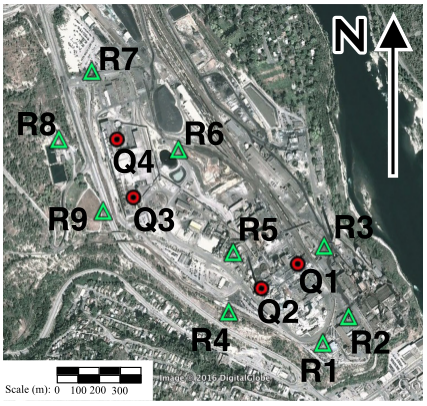
\includegraphics[scale=0.36]{BCtrail}
\ChangeFont
\end{figure}

\end{columns}
\end{frame}




\begin{frame}{Mathematical Model}
\begin{equation*}
\partial_{t} c(\textbf{x},t)+\nabla\cdot(\textbf{u}(\textbf{x},t)c+\textbf{S}(\textbf{x},t)\nabla c)
=q(\textbf{x},t)\qquad\text{on }\mathbb{R}^{2}\times\mathbb{R}_{\geq 0}\times(0,T).
\end{equation*}
\begin{itemize}
\item $\textbf{u}(\textbf{x},t)=(u_{x}(z,t),u_{y}(z,t),u_{set})$ 
(Wind velocity field)
\item $\|(u_{x},u_{y})\|_{2}\propto\left(\frac{z}{z_{r}}\right)^{\gamma}$,
\item $\textbf{S}=diag(s_{x},s_{y},s_{z})$ (Eddy diffusion matrix),
\item $s_{z}=f(L,z_{cut})$,
\item $s_{x}=s_{y}=g(z_{i},L)$, with $z_{i}$ Mixing layer height.
\end{itemize}
\end{frame}



\begin{frame}{Boundary Conditions}

\begin{itemize}
\item Far-field boundary condition
\begin{equation*}
c(\textbf{x},t)\rightarrow 0 as \|x\|\rightarrow \infty
\end{equation*}

\item Robin boundary conditions at $z=0$
\begin{equation*}
\left(u_{set}c+s_{z}\frac{\partial c}{\partial z}\right)|{z=0}=u_{dep}c|_{z=0}
\end{equation*}


\end{itemize}
\end{frame}


\begin{frame}


\begin{itemize}
\item Concentration and deposition are related via

\begin{equation}\label{eqnw}
w(x,y,T)=\int_{0}^{T}c(x,y,0,t)u_{set}dt.
\end{equation}

\begin{equation*}
F(x_{i},y_{i},T)=\int_{R_{i}}w(x,y,T)dxdy\approx w(x_{i},y_{i},T)\Delta A,
\end{equation*}
\item $\Delta A$ is the cross-sectional area of the dust-fall jar
\item $T$ is taken to be one month.
\end{itemize}

\end{frame}


\begin{frame}
\begin{itemize}

\item Numerical solution of the concentration $c$ was obtained via 
a finite volume solver\footnote{Hosseini, Bamdad and Stockie, J.M. Estimating airborne particulate emissions using a finite-volume
forward solver coupled with a Bayesian inversion approach.}
using a 30x30 resolution grid on the domain.



\item Solving for one set of parameters can take up to half an hour.
\end{itemize}

\textbf{Conclusion:} Finding the deposition $F$  is computationally very expensive.
\end{frame}






\begin{frame}{Roadmap}
\begin{enumerate}
\item Find a surrogate for $F$,
\item Locate the optimal points to evaluate $F$ so that the surrogate is accurate,
\item See if it is possible to do dimensionality reduction,
\item Use the Bayesian framework to obtain the posterior distribution of the parameters 
in the light of the experimental data,
\item Perform inference on the posterior using numerical methods.
\end{enumerate}
\end{frame}  


\section{Setting up the Problem}

\subsection{Finding a Surrogate for $F$}


\begin{frame}{Gaussian Process}
\begin{dfn} 
A Gaussian process (GP) is a collection of random variables $\{g(x)\}_{x\in A}$, for some set $A$,
possibly uncountable,
 such that any finite subset of random variables
 $\{g(x_{k})\}_{k=1}^{N}\subset\{g(x)\}_{x\in A}$ for
$\{x_{k}\}_{k=1}^{N}\subset A$ are jointly Gaussian.

A GP is completely defined by its mean m(x) and covariance operator k(x,x'):
\begin{equation*}
m(x)=\mathbb{E}(g(x)),
\end{equation*}
\begin{equation*}
k(x,x')=\mathbb{E}\left((x-m(x))(x'-m(x'))\right).
\end{equation*}

\end{dfn}
\end{frame}

%In this section you introduce everything that is related to GPs








\begin{frame}
\frametitle{Gaussian Process as Interpolator}
\begin{figure}
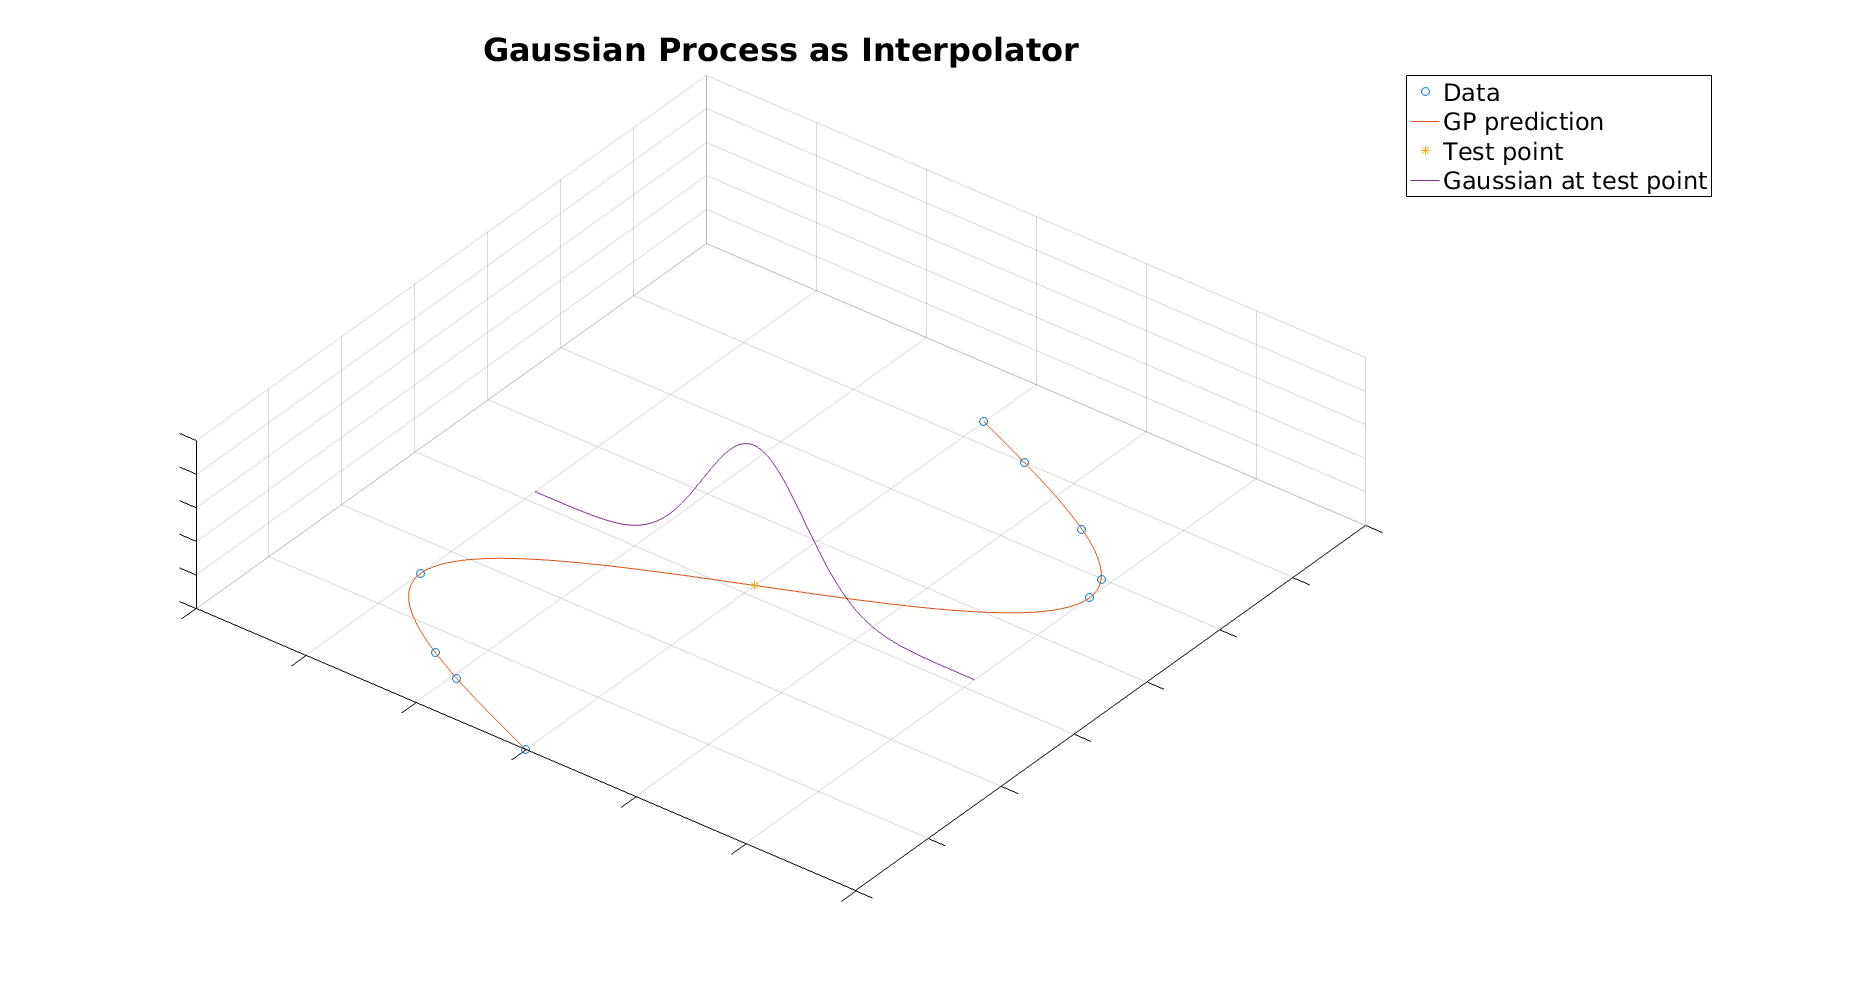
\includegraphics[scale=0.25]{./codes/Gp_interpolation.png}
\end{figure}

\end{frame}


\begin{frame}{Interpolation with Real Data}


\begin{figure}
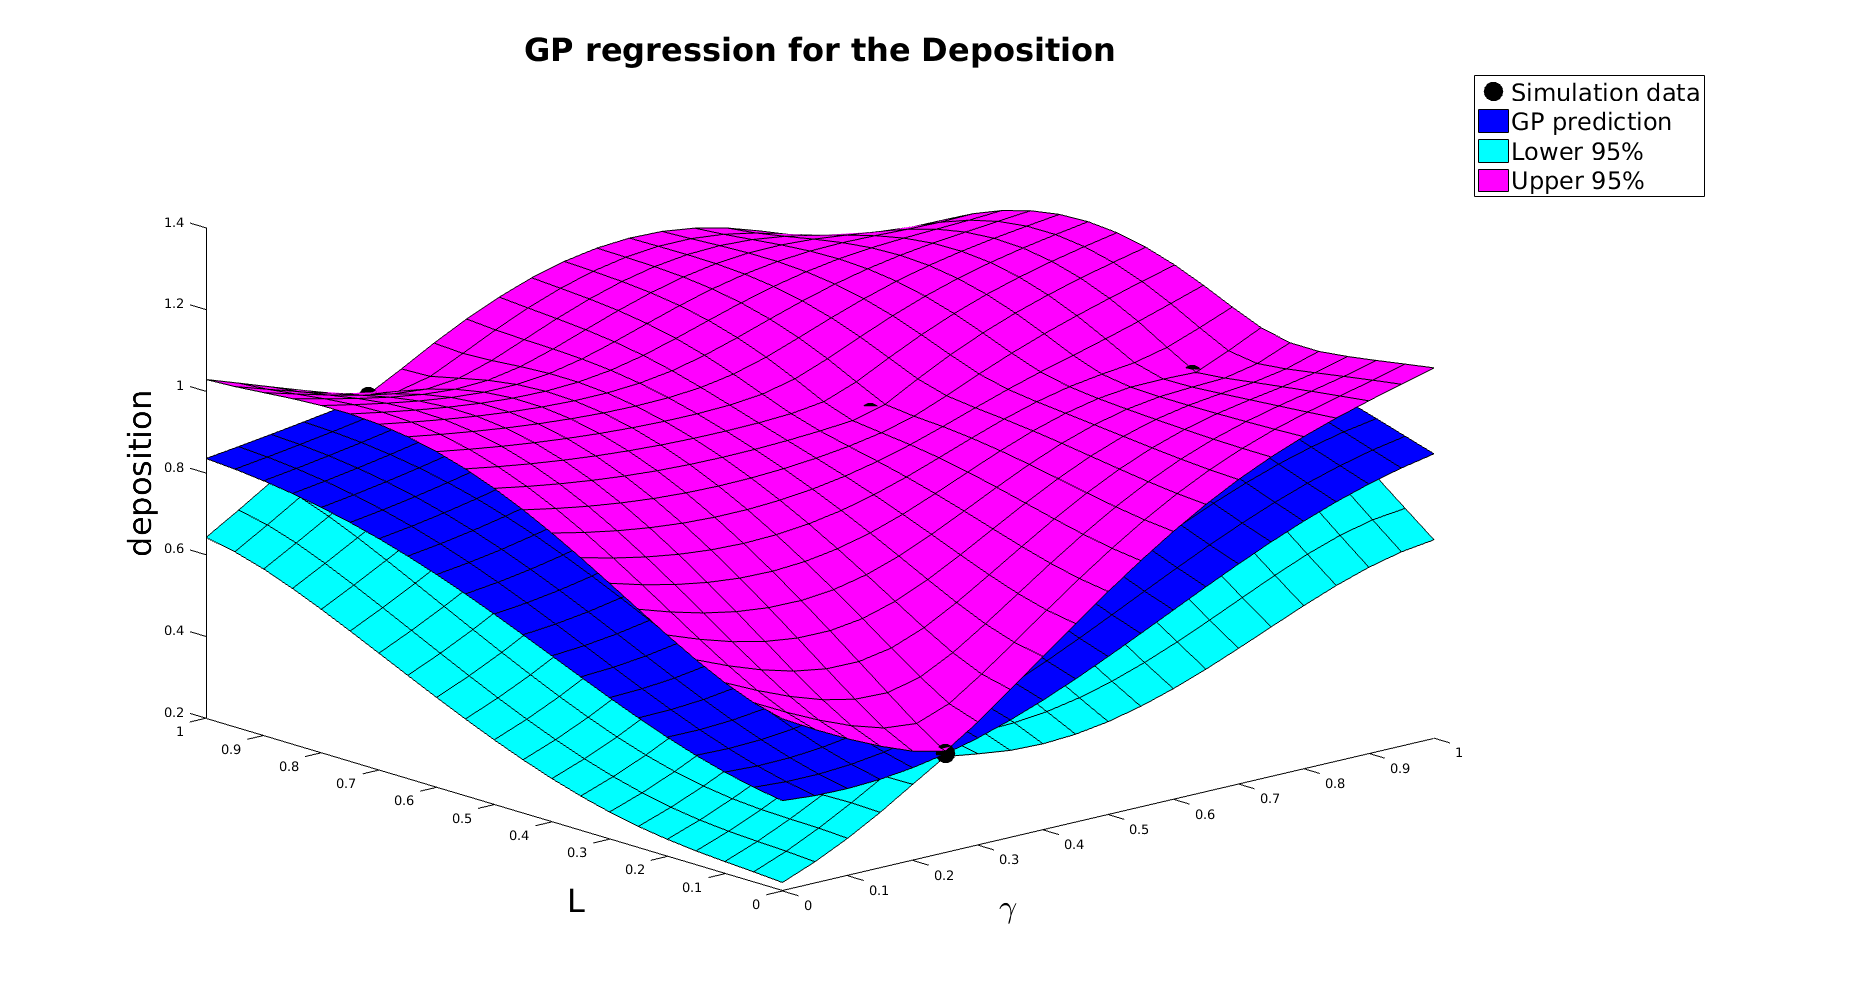
\includegraphics[scale=0.2]{./codes/GP_regression.png}
\end{figure}

\end{frame}

\subsection{Optimizing the Surrogate Interpolation Capabilities}


\begin{frame}{Why Experimental Design}
\begin{figure}
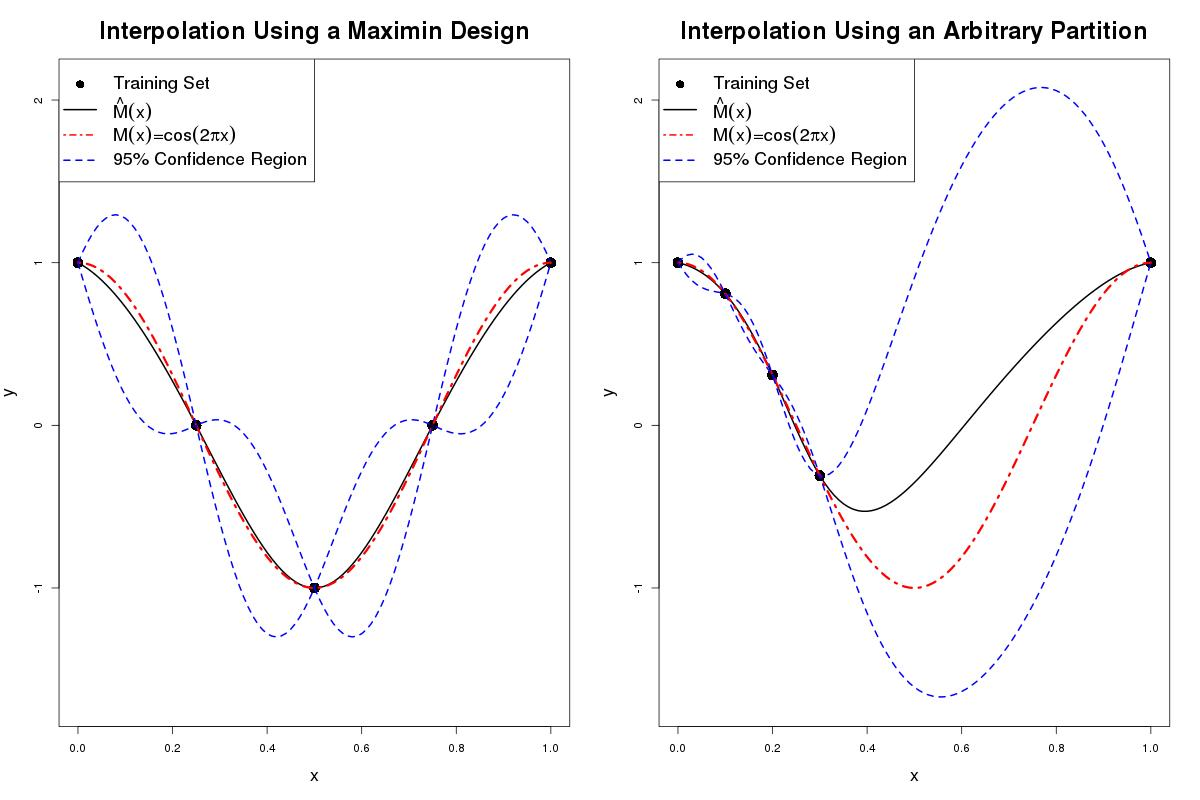
\includegraphics[scale=0.2]{../FigChap2/partitionComparison.jpg}
\end{figure}

\end{frame}

\begin{frame}{Maximin Design}

Given $T\subset\mathbb{R}^{n}$ and a subset $S$ of $T$, 
with finite (fixed) cardinality, say $|S|=n$.
A maximin distance design $S^{o}$ is a collection of points of $T$  such that
\begin{equation*}
\max_{(S\subset T,\text{ }|S|=n)}\min_{(s,s'\in S)}\|s-s'\|=\min_{s,s'\in S^{o}}\|s-s'\|=max!,
\end{equation*}
\end{frame}

\begin{frame}{Example of a Design}
\begin{figure}
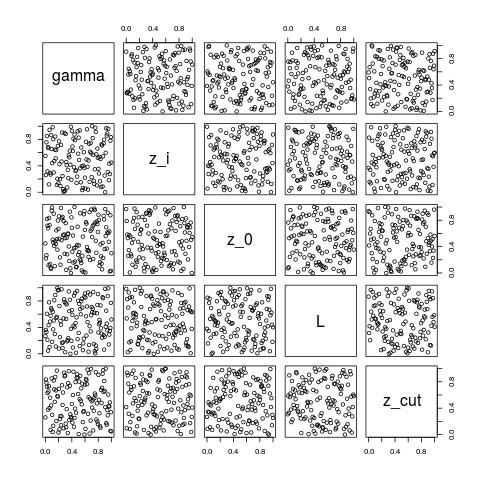
\includegraphics[scale=0.35]{./codes/experimental_design128.png}
\end{figure}

\end{frame}
%Here comes the part when you talk about design of experiments

\subsection{Reducing the Complexity of the Model}




\begin{frame}
\frametitle{Sensitivity Analysis}
\begin{columns}[c]
\column{0.4\textwidth}
\ChangeFont
\begin{itemize}
\item $\gamma$: Fitting parameter for the z dependence of the velocity.
\item $z_{0}$: Roughness length.
\item $z_{i}$: Mixing layer height.
\item $L$: Monin-Obukhov length.
\item $z_{cut}$: cutoff height.
\end{itemize}

\column{2.5in}
\begin{figure}
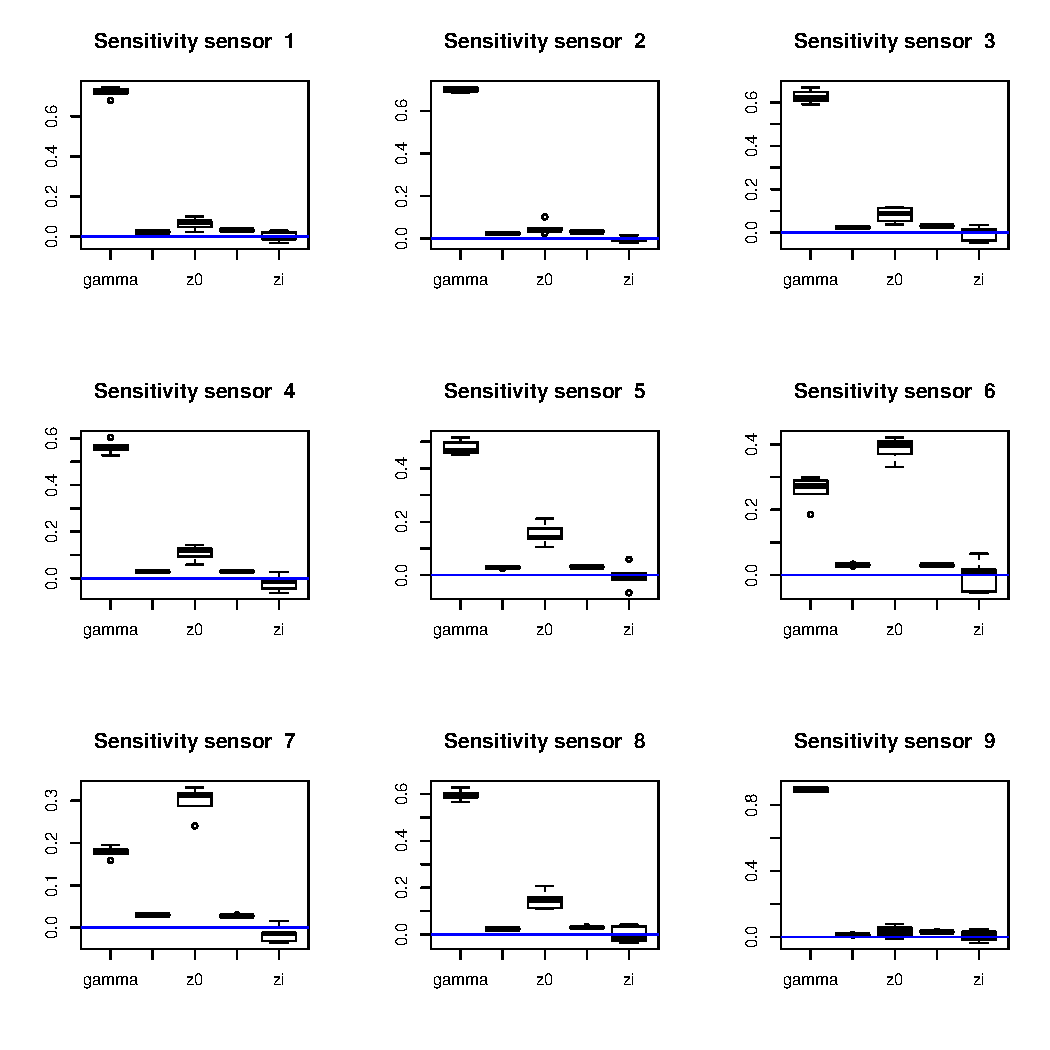
\includegraphics[scale=0.35]{../FigChap4/sensitivityPlot.pdf}
\end{figure}
\end{columns}

\end{frame}



\begin{frame}
\frametitle{What About the Sources?}

\begin{dfn}
The deposition behaves linearly  with respect to the values of the 4  sources,
hence
\begin{equation*}
\begin{bmatrix}
R_{1} \\
R_{2} \\
\vdots\\
R_{9}
\end{bmatrix}=\mathcal{A}(\gamma,z_{0},L)
\begin{bmatrix}
q_{1}\\
\vdots\\
q_{4}
\end{bmatrix}
\end{equation*}
To evaluate the matrix $\mathcal{A}(\gamma,z_{0},L)$ we approximate its entries by Gaussian process
and create a surrogate $A(\gamma,z_{0},L)$.
\end{dfn}
\end{frame}



\section{Introducing the Bayesian Framework}

\begin{frame}{Bayes' Rule}

Given a probability space $(\Omega,\mathscr{F},\p)$ and two events $A,B\in\mathscr{F}$, with $\p(B)\neq 0$,
we define the conditional probability of $A$ given $B$ by

\begin{equation*}
\p(A|B)=\frac{\p(A\cap B)}{\p(B)}.
\end{equation*}


With the definitions above, we are now in a position to state Bayes' fomula as
\begin{equation}\label{eqnBayes}
\post(A|B)\propto\like(B|A)\prior(A).
\end{equation}

\end{frame}



\begin{frame}{Looking at the Stochastic Model}
\begin{dfn}
To account for the uncertainties in the model and in the experimental measurements we propose the model
\begin{equation*}
\begin{bmatrix}
R_{1} \\
R_{2} \\
\vdots\\
R_{9}
\end{bmatrix}=A(\gamma,z_{0},L)
\begin{bmatrix}
q_{1}\\
\vdots\\
q_{4}
\end{bmatrix}+\epsilon,\qquad\text{where }\epsilon\sim \mathcal{N}(0,\lambda_{\epsilon} I_{9\times 9})
\end{equation*}
\end{dfn}
\end{frame}


\begin{frame}
\frametitle{Probabilistic Model}

\begin{dfn}
Our goal is to estimate the values of $\omega:=(\gamma,z_{0},L)$ and 
$q:=(q_{1},q_{2},q_{3},q_{4})$ given the measurements
$\vec{R}$. Mathematically we want to estimate:

\begin{equation*}
\post(\omega,q|\vec{R})\propto
\underbrace{\like(\vec{R}|\omega,q)\prior(\omega)\prior(q)}_{\text{Assuming $p$ and $q$ independent}}
\end{equation*}
We assume $\omega\sim Uniform$ over the domain of definition of the parameters.
 
\end{dfn}
\end{frame}

\begin{frame}
\frametitle{What About $q$?}
\begin{itemize}
\item $q_{k}>0$ for $k=1,2,3,4$.
\item If we trust the engineers the most likely value for $q$ is the engineers estimate and the 
true value cannot be very far away from those estimates.
\end{itemize}

\begin{table}[H]
\centering
\begin{tabular}{|c|c|}
\hline 
Source & Estimated Emission Rate {[}ton/yr{]}\tabularnewline
\hline 
\hline 
$q_{1}$ & 35\tabularnewline
\hline 
$q_{2}$ & 80\tabularnewline
\hline 
$q_{3}$ & 5\tabularnewline
\hline 
$q_{4}$ & 5\tabularnewline
\hline 
\end{tabular}
\end{table}
\end{frame}

\begin{frame}
\frametitle{Choosing a Prior for $q$}
\begin{columns}[c]
\column{2.2in}
A consistent assumption is $q_{k}\sim Ga(\alpha_{k},\beta_{k})$,for $k=1,2,3,4$,
the following conditions that define $\alpha_{k}$ and $\beta_{k}$ for all $k$ uniquely.

\begin{itemize}
\item $\beta_{k}(\alpha_{k}-1)=q_{eng,k}$
\item $qgamma(0.99,\alpha_{k},\beta_{k})=3q_{eng,k}$
\end{itemize}
\column{1.5in}
\begin{figure}
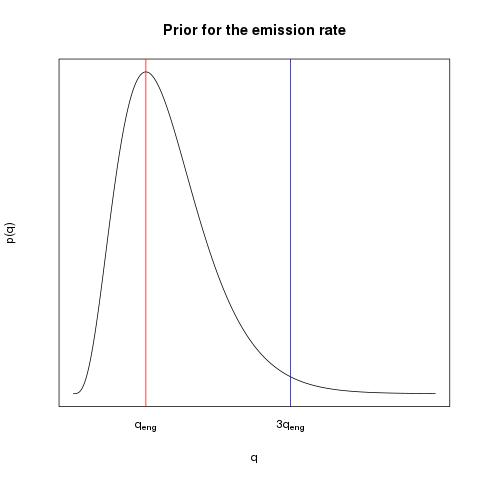
\includegraphics[scale=0.3]{gamma_generic}
\end{figure}
\end{columns}
\end{frame}


\begin{frame}{Likelihood}


Recall that $\epsilon\sim\mathcal{N}(0,\lambda_{\epsilon}I_{9\times 9})$ then

\begin{itemize}
\item $\p(\epsilon)\propto\exp\left(-\frac{\|\epsilon\|_{2}^{2}}{2\lambda_{\epsilon}^{2}}\right)$
\item $\like(\vec{R}|\omega,q)\propto
\exp\left(-\frac{1}{2\lambda_{\epsilon}^{2}}\|\vec{R}-A(\omega)q\|^{2}_{2}\right)$
\end{itemize}
\end{frame}

\begin{frame}
\frametitle{Calculating the Posterior}
\begin{itemize}
\item $\like(\vec{R}|\omega,q)\propto
\exp\left(-\frac{1}{2\lambda_{\epsilon}^{2}}\|\vec{R}-A(\omega)q\|^{2}_{2}\right)$
\item $\prior(q_{k})\propto q_{k}^{\alpha_{k}-1}\exp(\beta_{k}q_{k})$
\item $\prior(\omega)\propto\textbf{1}_{[0.1,0.6]\times[0,2]\times[-600,0]}$
\end{itemize}
\bigskip
Then
\begin{equation*}
\post(\omega,q|\vec{R})\propto\like(\vec{R}|\omega,q)\prior(\omega)\prior(q)
\end{equation*}
\end{frame}




\section{Decoding the Posterior}


\begin{frame}{Sampling From a Probability Distribution}
%
\begin{algorithm}[H]
\ChangeFont
\caption{Metropolis-Hastings Algorithm}
\begin{algorithmic}[1]\label{algMH}
\State pick a point $q_{1}$ in the support of the distribution
\For{j=2:N}
\State Draw $u\sim U([0,\alpha])$
\State $q_{j}\leftarrow q_{j-1}+u$
\State $\beta\leftarrow\min(1,\frac{\post(q_{j}|D)}{\post(q_{j-1}|\y)})$
\State Draw $w\sim U([0,1])$
\If{$w<\beta$}
\State $q_{j-1}=q_{j}\qquad$   (Accept the move)
\Else
\State $q_{j-1}=q_{j-1}\qquad$ (Reject the move)
\EndIf
\EndFor
\end{algorithmic}
\end{algorithm}
\end{frame}

\begin{frame}{Setting $\lambda_{\epsilon}$}
We define
\begin{equation*}
J(\lambda_{\epsilon})=\frac{1}{2}\int\left(\|A(p)q-\vec{R})\|_{2}+\|q-q_{est}\|_{2}\right)d\post^{\lambda_{\epsilon}},
\end{equation*}

and choose a minimizer of $J$ 
\begin{equation*}
\hat{\lambda_{\epsilon}}=argmin\text{ } J(\lambda_{\epsilon}).
\end{equation*}
%Finally explain the MCMC techniques

\end{frame}


\begin{frame}{Calculating $J$}
\begin{figure}
\centering
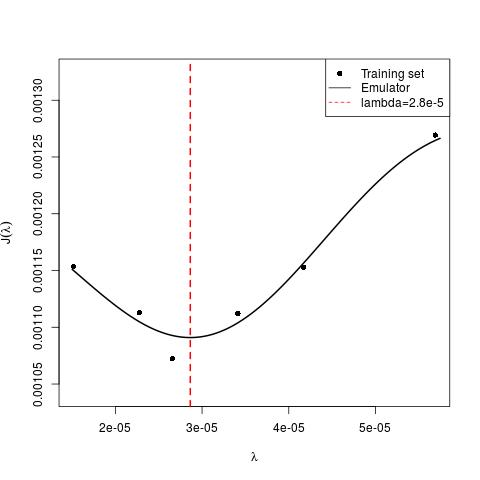
\includegraphics[scale=0.35]{../FigChap4/lambdaEmul}
\end{figure}


\end{frame}

\begin{frame}{Histograms for the Parameters}

\begin{figure}
\centering
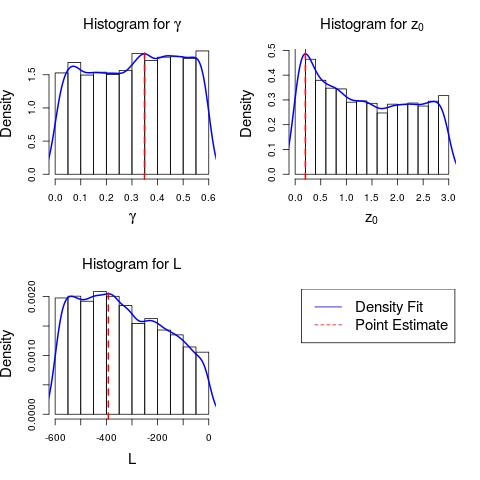
\includegraphics[scale=0.35]{./codes/histogramsI.jpg}
%\caption{Histograms for the marginal distribution for each of the seven variables
%in the support of the posterior density.}
\end{figure}
\end{frame}


\begin{frame}{Histograms for the Sources}
\begin{figure}
\centering
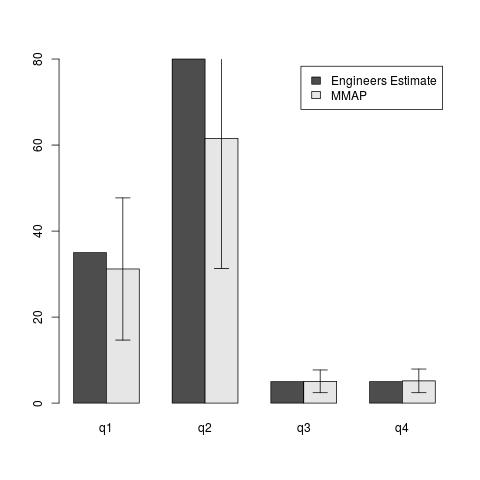
\includegraphics[scale=0.35]{../FigChap4/histogramsII}
\end{figure}
\end{frame}



\begin{frame}{Results for the Parameters}

\begin{table}
\centering
\begin{tabular}{|c|c|c|c|}
\hline 
Parameter & Point Estimate & $68\%$ Confidence Interval\tabularnewline
\hline 
\hline 
$\gamma$ &  0.3478 & $[0.1498,0.5458]$\tabularnewline
\hline 
$z_{0}$ & 0.0811 & $[0,1.5781]$\tabularnewline
\hline 
$L$  & -379.45 & $[-195.86,-563.04]$\tabularnewline
\hline 
\end{tabular}
\end{table}

\end{frame}

\begin{frame}{Results for the Sources}
\begin{figure}
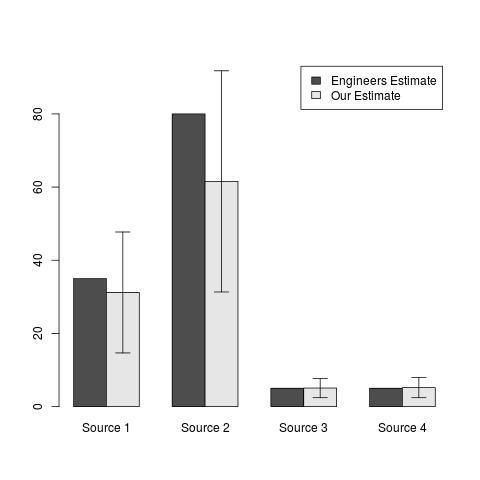
\includegraphics[scale=0.4]{../FigChap4/qUncertainty}
\end{figure}
\end{frame}


\begin{frame}{Comparison with Related Work}
\begin{figure}
\begin{columns}[c]
\column{.5\textwidth}
%\begin{textblock*}{5cm}(5cm,5cm)
\begin{figure}
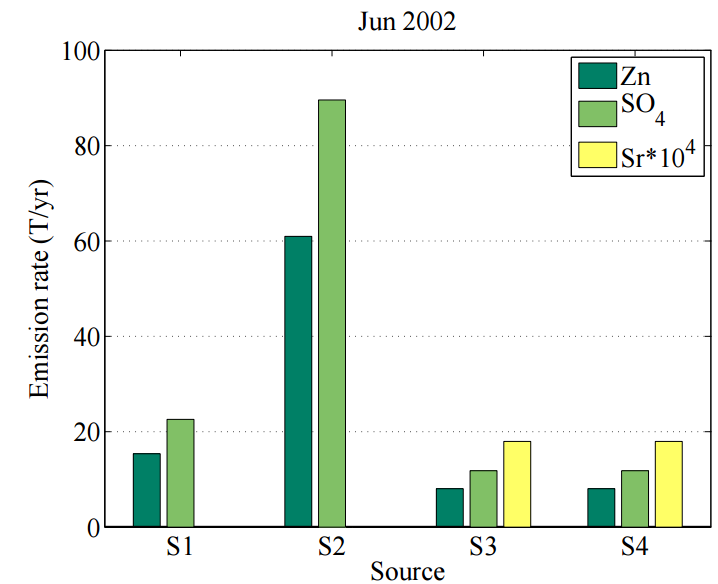
\includegraphics[scale=0.25]{Stockie_Lushi}
\caption{Hosseini, Bamdad and Stockie, J.M. Estimating airborne particulate emissions using a finite-volume
forward solver coupled with a Bayesian inversion approach.}
\end{figure}
%\end{textblock*}
\column{.5\textwidth}
\begin{figure}
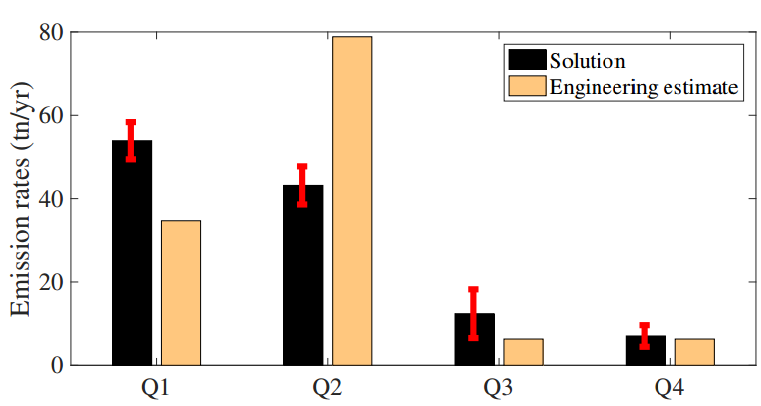
\includegraphics[scale=0.28]{Hosseini}
\caption{Lushi, E. and Stockie, J.M. An inverse Gaussian plume approach for estimating atmospheric
pollutant emissions from multiple point sources}
\end{figure}
\end{columns}
\end{figure}
\end{frame}


\begin{frame}{Conclusions}
\begin{itemize}
\item We have developed a method to cheaply estimate parameters in computationally expensive models.
\item Instead of trial and error, we propose a methodology that allows to estimate
parameters in complex models using experimental data.
\item Besides a point estimate we are able to obtain a confidence interval for it.
\item Our results qualitatively agree with previous results.
\end{itemize}


\end{frame}


\end{document}
